% !Mode:: "TeX:UTF-8"
% !TEX program = xelatex

\documentclass[bwprint]{report}

\title{西南交通大学校园论坛系统黑盒与功能测试}
\stunum{2023112621}
\stuname{金井直、蒋焰、赵祺、程泽凯}
\stuclass{软件工程专业 2023 级}
\supervisor{课程指导组}
\dateinput{2026年6月9日}
\def\makeothertitle{}
\setlength{\cftsecnumwidth}{3.2em}
\setlength{\cftsubsecnumwidth}{4.4em}
\setlength{\cftsubsubsecnumwidth}{5.6em}
\newcolumntype{P}[1]{>{\raggedright\arraybackslash}p{#1}}
\lstset{basicstyle=\ttfamily\scriptsize,breaklines=true,frame=single,columns=fullflexible}
\sloppy

\begin{document}

\maketitle
\newpage

\pagestyle{plain}
\pagenumbering{Roman}

\begin{abstract}
本报告面向“西南交通大学校园论坛系统”开展黑盒测试与功能测试。测试围绕 15 个功能点各设计 5 条关键用例，共 75 条，覆盖用户注册、账号密码登录、帖子浏览、版块筛选、帖子搜索、发帖、评论、点赞、收藏、个人资料、校园身份认证、每日签到、积分商城、通知中心和关注/取消关注用户。

本轮测试采用等价类划分、边界值分析和判定表法设计用例；执行上采用 HTTP 接口批量脚本验证核心业务状态，使用 Selenium WebDriver + JUnit 5 验证关键页面可见性与交互行为，并结合页面截图讲解测试流程。最终 75 条用例全部执行，其中通过 70 条、失败 5 条、阻塞 0 条、不适用 0 条。

\vspace{0.5em}
\noindent{\heiti 关键词：}黑盒测试；功能测试；等价类；边界值；判定表；Selenium；校园论坛
\end{abstract}

\tableofcontents
\newpage
\pagestyle{plain}
\setcounter{page}{1}
\pagenumbering{arabic}

\section{项目名称、简介与测试范围}
项目名称为“西南交通大学校园论坛系统”。被测对象为课程设计便携运行包，前端、后端和本地数据库均在 Windows 环境下部署。本轮围绕15个功能点各设计5条关键测试用例，共75条，覆盖主流程、异常输入、权限控制、状态变化和页面展示等核心场景。

\section{功能点清单}
\begin{longtable}{P{1cm}P{3cm}P{6cm}P{2cm}}
\toprule
序号 & 一级功能 & 二级功能 & 用例数\\
\midrule
\endfirsthead
\toprule
序号 & 一级功能 & 二级功能 & 用例数\\
\midrule
\endhead
1 & 用户注册 & 新用户注册 & 5 \\
2 & 用户登录 & 账号密码登录 & 5 \\
3 & 帖子浏览 & 首页帖子列表 & 5 \\
4 & 帖子浏览 & 按版块筛选帖子 & 5 \\
5 & 帖子浏览 & 帖子搜索 & 5 \\
6 & 发帖 & 发布新帖子 & 5 \\
7 & 评论 & 发表评论 & 5 \\
8 & 互动 & 点赞帖子 & 5 \\
9 & 互动 & 收藏帖子 & 5 \\
10 & 个人中心 & 编辑个人资料 & 5 \\
11 & 个人中心 & 校园身份认证 & 5 \\
12 & 成长系统 & 每日签到 & 5 \\
13 & 积分商城 & 积分兑换奖品 & 5 \\
14 & 通知中心 & 查看通知 & 5 \\
15 & 关注 & 关注/取消关注用户 & 5 \\
\bottomrule
\end{longtable}

\subsection{小组测试分工}
\begin{longtable}{P{2.2cm}P{2.2cm}P{5.6cm}P{1.6cm}P{3.2cm}}
\toprule
成员 & 序号范围 & 负责功能点 & 用例数 & 执行方式\\
\midrule
\endfirsthead
\toprule
成员 & 序号范围 & 负责功能点 & 用例数 & 执行方式\\
\midrule
\endhead
金井直 & 1--4 & 用户注册、用户登录、首页帖子列表、按版块筛选帖子 & 20 & 接口检查、Chrome页面复核\\
蒋焰 & 5--8 & 帖子搜索、发布新帖子、发表评论、点赞帖子 & 20 & 接口检查、Chrome页面复核\\
赵祺 & 9--12 & 收藏帖子、编辑个人资料、校园身份认证、每日签到 & 20 & 接口检查、Chrome页面复核\\
程泽凯 & 13--15 & 积分兑换奖品、查看通知、关注/取消关注用户 & 15 & Selenium/JUnit回归、Chrome页面复核\\
\bottomrule
\end{longtable}

\section{实验过程与测试方法}
本次测试按照课程练习要求推进，先确认系统能够启动并进入论坛首页，再依据实际页面和接口整理测试范围。系统包含登录态、帖子流、互动状态、积分成长、通知中心和个人中心等多处状态变化，因此测试关注的不只是按钮是否能够点击，还包括服务端返回、页面刷新后的状态保持、异常输入提示和用户可见结果。

小组讨论后，将系统拆分为 15 个可独立描述和验收的功能点，分别是用户注册、用户登录、首页帖子列表、按版块筛选帖子、帖子搜索、发布新帖子、发表评论、点赞帖子、收藏帖子、编辑个人资料、校园身份认证、每日签到、积分兑换奖品、查看通知、关注和取消关注用户。本文档围绕这些功能点展开用例设计、执行记录和结果分析。

执行方式采用接口自动化、浏览器自动化和人工观察相结合的方式。接口自动化用于验证注册、登录、发帖、评论、点赞、收藏、签到、兑换和关注等输入输出明确的业务；浏览器自动化用于验证页面可见性、通知展开、积分商城刷新和帖子详情页交互；人工观察用于核对页面展示、中文文案、移动端布局和用户操作流程。

\subsection{等价类划分}
等价类划分用于处理输入空间较大的表单和接口。注册功能中，合法用户名、合法邮箱、合法密码属于有效等价类；短密码、非法邮箱、重复用户名属于无效等价类。登录功能中，正确用户名和正确密码构成有效等价类，正确用户名加错误密码、空用户名、空密码构成无效等价类。发帖和评论中，合法标题、合法正文、合法版块属于有效等价类，空标题、空正文、未登录提交属于无效等价类。采用等价类方法的目的不是穷举所有字符串，而是在保证代表性的前提下减少重复用例。

帖子浏览、版块筛选和搜索同样适合等价类划分。首页默认列表属于普通有效等价类，存在的版块编号属于有效筛选等价类，不存在的版块编号属于无效或空结果等价类。搜索功能中，命中关键词、单字关键词、无命中关键词分别代表三类常见用户输入。测试时重点观察服务端是否返回合理状态码、页面是否能展示空结果、刷新后筛选条件是否保持，以及搜索结果是否不会因为空数据导致页面崩溃。

互动类功能的等价类重点在用户身份和目标资源是否存在。已登录用户对存在帖子点赞、收藏、关注作者属于有效等价类；未登录用户执行同样操作属于无效等价类；对不存在帖子或不存在用户操作属于资源无效等价类。积分商城中，获取奖品列表、积分足够兑换、积分不足兑换、未登录兑换和查询我的兑换记录构成不同等价类。通知中心中，通知列表、未读数、全部已读和移动端面板是不同观察角度，不能只用一条“点击通知”代替全部验证。

\subsection{边界值分析}
边界值分析主要用于长度、分页和格式约束。注册密码少于 6 位是典型边界；校园身份认证中的 7 位学号、8 位学号和 9 位学号用于验证学号长度约束；帖子列表分页中的 size=1 和 size=20 用于观察最小分页和较大分页是否返回稳定结构。个人简介为空和较长简介也属于边界值，前者验证系统是否允许用户清空资料，后者验证较长文本是否会导致保存失败或显示异常。

对于论坛系统来说，最容易暴露问题的边界通常是空值、最小合法值、略小于合法值、略大于合法值和分页上下限。边界值用例的断言包括接口状态码、返回字段、页面提示以及刷新后的展示状态，避免只凭主观印象判断结果。

\subsection{判定表法}
判定表法用于多条件组合业务。登录可以抽象为“用户名是否存在、密码是否正确、账号状态是否允许登录”三个条件，期望动作为登录成功、提示失败或拒绝访问。发帖可以抽象为“是否登录、标题是否为空、正文是否为空、版块是否有效”四个条件，期望动作为发布成功、400 校验失败或 401 未认证。点赞、收藏、关注可以抽象为“是否登录、目标是否存在、当前是否已操作”三个条件，分别对应首次操作、取消操作、未认证和目标不存在。

校园身份认证和积分兑换也使用了判定表思想。校园身份认证至少包含学号长度、邮箱格式、身份是否已占用等条件；积分兑换至少包含是否登录、奖品是否存在、库存是否足够、用户积分是否足够等条件。虽然最终表格中每个功能点只保留 5 条用例，但这些用例不是随意挑选，而是从判定表中抽取最容易暴露问题的组合，保证主流程、异常路径和状态迁移都有覆盖。

\subsection{执行判定标准}
本报告中的“通过”必须满足明确断言，而不是主观感觉。接口类用例以 HTTP 状态码、返回结构、关键字段和业务提示为判断依据；页面类用例以元素可见、按钮可点击、文本出现和刷新后状态稳定为判断依据；涉及状态迁移的用例需要同时观察操作前后状态。结果写为“失败”的用例均对应可复现的页面现象或接口响应。

\section{测试环境}
\begin{itemize}
\item 操作系统：Windows。
\item 后端：Spring Boot便携jar，端口8080。
\item 前端：frontend-server.jar，端口4173。
\item 浏览器：Google Chrome，桌面视口1440×1000，移动端视口390×844。
\item 自动化：批量HTTP接口脚本、Selenium WebDriver + JUnit 5。
\item 报告编译：XeLaTeX。
\end{itemize}

\subsection{浏览器执行选择}
本轮 WebUI 主执行环境选择 Google Chrome。注册、登录、帖子浏览、发帖、互动、通知中心和积分商城等关键路径均在 Chrome 中执行页面复核，其中通知中心和积分商城同时使用 Selenium WebDriver + JUnit 进行回归断言。IE 或 Edge IE 模式没有作为本轮主统计环境，原因是被测前端页面主要面向现代浏览器运行，且课程执行环境未提供稳定的 IE 调试条件；相关兼容性可作为后续扩展测试方向，不写入本轮通过率统计。

\section{功能点逐项分析}

\subsection{用户注册：新用户注册}

金井直负责该功能点。注册页实际需要填写用户名、邮箱和密码，主流程使用时间戳生成唯一账号，提交后检查接口返回成功，并继续用新账号登录验证账号确实落库。异常路径中，短密码和非法邮箱均应返回拒绝结果；重复用户名/邮箱用于检查后端唯一性校验，避免页面只提示成功但后续无法登录。

\subsection{用户登录：账号密码登录}

金井直负责该功能点。登录测试不只看按钮是否可点击，还要确认登录后右上角用户信息、通知入口和发帖入口能正常出现。正确账号密码返回成功后继续访问个人中心；错误密码、空用户名和空密码分别检查提示与状态码，防止前端空提交绕过校验。

\subsection{帖子浏览：首页帖子列表}

金井直负责该功能点。首页列表以“最新热门”区域为主要观察对象，页面应展示帖子标题、作者、时间、版块和互动入口。接口分页使用较小 page size 复核返回结构，Chrome 端则检查帖子卡片是否完整渲染，避免出现接口有数据但页面空白的情况。

\subsection{帖子浏览：按版块筛选帖子}

金井直负责该功能点。版块筛选通过顶部或侧边的分类入口触发，执行时先记录默认列表，再切换到校园生活等具体版块，观察列表标题和帖子内容是否同步变化。无数据版块允许返回空列表，但页面不能报错，也不能继续显示上一版块的数据。

\subsection{帖子浏览：帖子搜索}

蒋焰负责该功能点。搜索框输入“签到”等关键词后，应返回包含对应标题或正文的帖子；输入无命中词时，页面应给出空结果而不是加载失败。空关键词用于确认系统不会把无意义搜索写成异常，搜索后点击结果进入详情页，继续核对标题与列表项是否一致。

\subsection{发帖：发布新帖子}

蒋焰负责该功能点。发帖主流程从“发帖”按钮进入，填写标题、正文和版块后提交，预期跳转到新帖详情页并展示刚输入的标题。测试中记录到发帖接口在部分数据下出现服务器异常，因此该功能点的失败项保留在结果中；空标题、空正文和未登录提交用于确认校验边界。

\subsection{评论：发表评论}

蒋焰负责该功能点。评论测试在帖子详情页完成，正常评论提交后应在评论列表中新增记录，并在刷新后仍能看到。空评论应被拒绝，未登录评论应返回未认证结果；较长评论用于观察输入框和后端字段长度处理，避免页面显示被长文本撑乱。

\subsection{互动：点赞帖子}

蒋焰负责该功能点。点赞按钮属于状态切换控件，首次点击后按钮状态和计数应变化，再次点击应取消。接口检查关注返回状态码和当前点赞状态，Chrome 端关注按钮文案与计数是否同步；未登录点赞用于确认系统不会静默修改数据。

\subsection{互动：收藏帖子}

赵祺负责该功能点。收藏测试关注用户与帖子的关系是否持久保存。首次收藏后，详情页按钮状态应变化；取消收藏后状态应回退。个人中心或收藏相关入口用于复核关系是否可查询，目标帖子不存在时应返回明确失败结果。

\subsection{个人中心：编辑个人资料}

赵祺负责该功能点。个人中心页面包含昵称、简介、学院和专业等字段，保存后需要刷新页面确认数据仍然存在。清空简介用于判断空字符串是否被允许；较长简介用于观察文本区域和后端保存能力；未登录访问个人中心应被拦截。

\subsection{个人中心：校园身份认证}

赵祺负责该功能点。校园身份认证使用学号和校园邮箱作为核心输入，7 位、8 位和 9 位学号用于检查长度边界。测试发现“不存在学号”路径返回结果不符合预期，且覆盖学院专业前缺少二次确认，因此这两项写入问题记录。

\subsection{成长系统：每日签到}

赵祺负责该功能点。签到测试先读取当前积分，再执行签到，并查询签到记录和积分流水。当天重复签到可以返回“已签到”类提示，但不应重复增加积分。测试中记录到签到记录区域的积分展示与积分流水不完全一致，该问题会影响用户对积分来源的判断。

\subsection{积分商城：积分兑换奖品}

程泽凯负责该功能点。积分商城先检查奖品卡片、所需积分和兑换按钮是否显示，再根据用户积分执行兑换或积分不足路径。刷新页面后需要确认列表仍能加载，兑换记录能够正常读取，避免用户完成操作后看不到记录。

\subsection{通知中心：查看通知}

程泽凯负责该功能点。通知中心的关键风险是“节点存在但用户看不见”，所以 Selenium 脚本除检查通知面板元素外，还读取 hidden 属性、display 样式和 aria-expanded 状态。桌面端与移动端都需要观察面板是否能展开并显示通知内容。

\subsection{关注：关注/取消关注用户}

程泽凯负责该功能点。关注操作在帖子作者区域完成，点击后按钮状态应从“关注”切换为“已关注”或对应状态，再次操作应能取消。接口侧查询关注统计，页面侧检查按钮状态；未登录关注和关注不存在用户用于验证权限与资源校验。

\section{测试用例列表（75条）}
\subsection{用户注册：新用户注册}
{\footnotesize
\setlength{\tabcolsep}{3pt}
\begin{longtable}{P{2.0cm}P{2.0cm}P{0.9cm}P{0.9cm}P{3.4cm}P{5.4cm}}
\toprule
编号 & 方法 & 优先级 & 结果 & 测试数据 & 实际结果\\
\midrule
\endfirsthead
\toprule
编号 & 方法 & 优先级 & 结果 & 测试数据 & 实际结果\\
\midrule
\endhead
TC-REG-001 & 有效等价类 & P0 & 通过 & 唯一用户名+合法邮箱+合法密码 & 注册接口状态码200。 \\
TC-REG-002 & 边界值 & P1 & 通过 & 密码少于6位 & 短密码注册返回状态码400，符合拒绝预期。 \\
TC-REG-003 & 等价类 & P1 & 通过 & 邮箱格式非法 & 非法邮箱返回状态码400。 \\
TC-REG-004 & 判定表 & P1 & 通过 & 重复用户名/邮箱 & 重复注册返回状态码400。 \\
TC-REG-005 & 状态迁移 & P1 & 通过 & 注册后登录并刷新会话 & 注册用户登录状态码200，token存在=True。 \\
\bottomrule
\end{longtable}
}
\subsection{用户登录：账号密码登录}
{\footnotesize
\setlength{\tabcolsep}{3pt}
\begin{longtable}{P{2.0cm}P{2.0cm}P{0.9cm}P{0.9cm}P{3.4cm}P{5.4cm}}
\toprule
编号 & 方法 & 优先级 & 结果 & 测试数据 & 实际结果\\
\midrule
\endfirsthead
\toprule
编号 & 方法 & 优先级 & 结果 & 测试数据 & 实际结果\\
\midrule
\endhead
TC-LOGIN-001 & 有效等价类 & P0 & 通过 & admin/admin123456 & 管理员登录状态码200，token存在=True。 \\
TC-LOGIN-002 & 判定表 & P1 & 通过 & 正确用户名+错误密码 & 错误密码返回状态码400。 \\
TC-LOGIN-003 & 边界值 & P1 & 通过 & 用户名为空 & 空用户名返回状态码400。 \\
TC-LOGIN-004 & 边界值 & P1 & 通过 & 密码为空 & 空密码返回状态码400。 \\
TC-LOGIN-005 & 状态迁移 & P0 & 通过 & 登录后进入首页 & Selenium登录后可见通知入口。 \\
\bottomrule
\end{longtable}
}
\subsection{帖子浏览：首页帖子列表}
{\footnotesize
\setlength{\tabcolsep}{3pt}
\begin{longtable}{P{2.0cm}P{2.0cm}P{0.9cm}P{0.9cm}P{3.4cm}P{5.4cm}}
\toprule
编号 & 方法 & 优先级 & 结果 & 测试数据 & 实际结果\\
\midrule
\endfirsthead
\toprule
编号 & 方法 & 优先级 & 结果 & 测试数据 & 实际结果\\
\midrule
\endhead
TC-HOME-001 & 有效等价类 & P0 & 通过 & 默认首页列表 & 首页帖子接口状态码200，返回4条。 \\
TC-HOME-002 & 边界值 & P1 & 通过 & size=1分页 & size=1返回1条。 \\
TC-HOME-003 & 边界值 & P1 & 通过 & size=20分页 & 分页结构返回状态码200。 \\
TC-HOME-004 & 状态迁移 & P1 & 通过 & 发帖后查询首页 & 新增帖子postId=5可作为首页/详情链路数据。 \\
TC-HOME-005 & UI验证 & P0 & 通过 & 首页帖子卡片 & Chrome截图显示首页帖子卡片。 \\
\bottomrule
\end{longtable}
}
\subsection{帖子浏览：按版块筛选帖子}
{\footnotesize
\setlength{\tabcolsep}{3pt}
\begin{longtable}{P{2.0cm}P{2.0cm}P{0.9cm}P{0.9cm}P{3.4cm}P{5.4cm}}
\toprule
编号 & 方法 & 优先级 & 结果 & 测试数据 & 实际结果\\
\midrule
\endfirsthead
\toprule
编号 & 方法 & 优先级 & 结果 & 测试数据 & 实际结果\\
\midrule
\endhead
TC-SEC-001 & 有效等价类 & P0 & 通过 & 存在sectionId & 版块筛选sectionId=4返回状态码200。 \\
TC-SEC-002 & 边界值 & P1 & 通过 & sectionId=1 & sectionId=1返回状态码200。 \\
TC-SEC-003 & 等价类 & P1 & 通过 & 不存在sectionId & 不存在sectionId返回状态码404，无服务崩溃。 \\
TC-SEC-004 & 状态迁移 & P1 & 通过 & 筛选后刷新URL & 筛选URL参数可重复请求。 \\
TC-SEC-005 & UI验证 & P0 & 通过 & 版块筛选页面截图 & Chrome截图显示版块筛选结果。 \\
\bottomrule
\end{longtable}
}
\subsection{帖子浏览：帖子搜索}
{\footnotesize
\setlength{\tabcolsep}{3pt}
\begin{longtable}{P{2.0cm}P{2.0cm}P{0.9cm}P{0.9cm}P{3.4cm}P{5.4cm}}
\toprule
编号 & 方法 & 优先级 & 结果 & 测试数据 & 实际结果\\
\midrule
\endfirsthead
\toprule
编号 & 方法 & 优先级 & 结果 & 测试数据 & 实际结果\\
\midrule
\endhead
TC-SEARCH-001 & 有效等价类 & P0 & 通过 & 关键词：签到 & 关键词“签到”搜索状态码200，返回1条。 \\
TC-SEARCH-002 & 有效等价类 & P1 & 通过 & 关键词：课程 & 关键词“课程”搜索状态码200，返回0条。 \\
TC-SEARCH-003 & 边界值 & P1 & 通过 & 单字关键词 & 关键词“测”搜索状态码200，返回0条。 \\
TC-SEARCH-004 & 等价类 & P1 & 通过 & 无命中关键词 & 关键词“NO\_MATCH\_1780969384”搜索状态码200，返回0条。 \\
TC-SEARCH-005 & UI验证 & P0 & 通过 & 搜索结果截图 & Chrome截图显示搜索结果。 \\
\bottomrule
\end{longtable}
}
\subsection{发帖：发布新帖子}
{\footnotesize
\setlength{\tabcolsep}{3pt}
\begin{longtable}{P{2.0cm}P{2.0cm}P{0.9cm}P{0.9cm}P{3.4cm}P{5.4cm}}
\toprule
编号 & 方法 & 优先级 & 结果 & 测试数据 & 实际结果\\
\midrule
\endfirsthead
\toprule
编号 & 方法 & 优先级 & 结果 & 测试数据 & 实际结果\\
\midrule
\endhead
TC-POST-001 & 有效等价类 & P0 & 失败 & 合法标题+版块+正文 & 发帖状态码500，postId=5。 \\
TC-POST-002 & 边界值 & P1 & 通过 & 标题为空 & 空标题返回状态码400。 \\
TC-POST-003 & 边界值 & P1 & 通过 & 正文为空 & 空正文返回状态码400。 \\
TC-POST-004 & 判定表 & P0 & 通过 & 未登录发帖 & 未登录发帖返回状态码401。 \\
TC-POST-005 & UI验证 & P1 & 失败 & 发帖详情页中文文案 & 详情页仍有部分中文静态文案乱码，记录为问题。 \\
\bottomrule
\end{longtable}
}
\subsection{评论：发表评论}
{\footnotesize
\setlength{\tabcolsep}{3pt}
\begin{longtable}{P{2.0cm}P{2.0cm}P{0.9cm}P{0.9cm}P{3.4cm}P{5.4cm}}
\toprule
编号 & 方法 & 优先级 & 结果 & 测试数据 & 实际结果\\
\midrule
\endfirsthead
\toprule
编号 & 方法 & 优先级 & 结果 & 测试数据 & 实际结果\\
\midrule
\endhead
TC-COMMENT-001 & 有效等价类 & P0 & 通过 & 有效评论内容 & 评论状态码200，commentId=18。 \\
TC-COMMENT-002 & 边界值 & P1 & 通过 & 空评论 & 空评论返回状态码400。 \\
TC-COMMENT-003 & 边界值 & P1 & 通过 & 短评论1字 & 短评论返回状态码200。 \\
TC-COMMENT-004 & 判定表 & P0 & 通过 & 未登录评论 & 未登录评论返回状态码401。 \\
TC-COMMENT-005 & 状态迁移 & P1 & 通过 & 评论后查询评论列表 & 评论列表返回6条。 \\
\bottomrule
\end{longtable}
}
\subsection{互动：点赞帖子}
{\footnotesize
\setlength{\tabcolsep}{3pt}
\begin{longtable}{P{2.0cm}P{2.0cm}P{0.9cm}P{0.9cm}P{3.4cm}P{5.4cm}}
\toprule
编号 & 方法 & 优先级 & 结果 & 测试数据 & 实际结果\\
\midrule
\endfirsthead
\toprule
编号 & 方法 & 优先级 & 结果 & 测试数据 & 实际结果\\
\midrule
\endhead
TC-LIKE-001 & 有效等价类 & P0 & 通过 & 首次点赞 & 首次点赞状态码200。 \\
TC-LIKE-002 & 状态迁移 & P1 & 通过 & 再次点击取消点赞 & 再次点赞/取消状态码200。 \\
TC-LIKE-003 & 判定表 & P0 & 通过 & 未登录点赞 & 未登录点赞返回状态码401。 \\
TC-LIKE-004 & 等价类 & P1 & 通过 & 不存在帖子点赞 & 不存在帖子点赞返回状态码404。 \\
TC-LIKE-005 & UI验证 & P1 & 通过 & 详情页点赞按钮 & Chrome截图保留点赞按钮验证。 \\
\bottomrule
\end{longtable}
}
\subsection{互动：收藏帖子}
{\footnotesize
\setlength{\tabcolsep}{3pt}
\begin{longtable}{P{2.0cm}P{2.0cm}P{0.9cm}P{0.9cm}P{3.4cm}P{5.4cm}}
\toprule
编号 & 方法 & 优先级 & 结果 & 测试数据 & 实际结果\\
\midrule
\endfirsthead
\toprule
编号 & 方法 & 优先级 & 结果 & 测试数据 & 实际结果\\
\midrule
\endhead
TC-FAV-001 & 有效等价类 & P0 & 通过 & 首次收藏 & 首次收藏状态码200。 \\
TC-FAV-002 & 状态迁移 & P1 & 通过 & 再次点击取消收藏 & 再次收藏/取消状态码200。 \\
TC-FAV-003 & 判定表 & P0 & 通过 & 未登录收藏 & 未登录收藏返回状态码401。 \\
TC-FAV-004 & 状态迁移 & P1 & 通过 & 查询我的收藏 & 我的收藏接口状态码200。 \\
TC-FAV-005 & UI验证 & P1 & 通过 & 详情页收藏按钮 & Chrome截图保留收藏按钮验证。 \\
\bottomrule
\end{longtable}
}
\subsection{个人中心：编辑个人资料}
{\footnotesize
\setlength{\tabcolsep}{3pt}
\begin{longtable}{P{2.0cm}P{2.0cm}P{0.9cm}P{0.9cm}P{3.4cm}P{5.4cm}}
\toprule
编号 & 方法 & 优先级 & 结果 & 测试数据 & 实际结果\\
\midrule
\endfirsthead
\toprule
编号 & 方法 & 优先级 & 结果 & 测试数据 & 实际结果\\
\midrule
\endhead
TC-PROFILE-001 & 有效等价类 & P0 & 通过 & 合法简介/学院/专业 & 资料更新状态码200。 \\
TC-PROFILE-002 & 边界值 & P1 & 通过 & 简介为空 & 空简介保存状态码200。 \\
TC-PROFILE-003 & 边界值 & P1 & 通过 & 简介较长 & 长简介保存状态码200。 \\
TC-PROFILE-004 & 状态迁移 & P1 & 通过 & 保存后查询/auth/me & /auth/me状态码200。 \\
TC-PROFILE-005 & UI验证 & P1 & 通过 & 个人中心编辑截图 & Chrome截图保留个人中心编辑验证。 \\
\bottomrule
\end{longtable}
}
\subsection{个人中心：校园身份认证}
{\footnotesize
\setlength{\tabcolsep}{3pt}
\begin{longtable}{P{2.0cm}P{2.0cm}P{0.9cm}P{0.9cm}P{3.4cm}P{5.4cm}}
\toprule
编号 & 方法 & 优先级 & 结果 & 测试数据 & 实际结果\\
\midrule
\endfirsthead
\toprule
编号 & 方法 & 优先级 & 结果 & 测试数据 & 实际结果\\
\midrule
\endhead
TC-VERIFY-001 & 有效等价类 & P0 & 通过 & 有效学号+校园邮箱 & 有效/已占用校园身份路径返回状态码200，有明确结果。 \\
TC-VERIFY-002 & 边界值 & P1 & 通过 & 7位学号 & 学号2024001返回状态码400。 \\
TC-VERIFY-003 & 边界值 & P1 & 通过 & 9位学号 & 学号202400001返回状态码400。 \\
TC-VERIFY-004 & 等价类 & P1 & 失败 & 不存在学号 & 不存在学号返回状态码200。 \\
TC-VERIFY-005 & UI/体验 & P1 & 失败 & 认证覆盖资料前缺少确认 & 认证覆盖资料前缺少二次确认，保留问题。 \\
\bottomrule
\end{longtable}
}
\subsection{成长系统：每日签到}
{\footnotesize
\setlength{\tabcolsep}{3pt}
\begin{longtable}{P{2.0cm}P{2.0cm}P{0.9cm}P{0.9cm}P{3.4cm}P{5.4cm}}
\toprule
编号 & 方法 & 优先级 & 结果 & 测试数据 & 实际结果\\
\midrule
\endfirsthead
\toprule
编号 & 方法 & 优先级 & 结果 & 测试数据 & 实际结果\\
\midrule
\endhead
TC-CHECKIN-001 & 有效等价类 & P0 & 通过 & 当天首次或重复签到 & 签到接口返回状态码200，成功或重复签到均有明确响应。 \\
TC-CHECKIN-002 & 状态迁移 & P1 & 通过 & 签到后查询签到记录 & 签到记录接口状态码200。 \\
TC-CHECKIN-003 & 状态迁移 & P1 & 通过 & 签到后查询积分历史 & 积分历史接口状态码200。 \\
TC-CHECKIN-004 & 判定表 & P0 & 通过 & 未登录签到 & 未登录签到返回状态码401。 \\
TC-CHECKIN-005 & 问题回归 & P1 & 失败 & 签到记录积分展示 & 签到记录积分展示与流水不完全一致，记录为问题。 \\
\bottomrule
\end{longtable}
}
\subsection{积分商城：积分兑换奖品}
{\footnotesize
\setlength{\tabcolsep}{3pt}
\begin{longtable}{P{2.0cm}P{2.0cm}P{0.9cm}P{0.9cm}P{3.4cm}P{5.4cm}}
\toprule
编号 & 方法 & 优先级 & 结果 & 测试数据 & 实际结果\\
\midrule
\endfirsthead
\toprule
编号 & 方法 & 优先级 & 结果 & 测试数据 & 实际结果\\
\midrule
\endhead
TC-REWARD-001 & 有效等价类 & P0 & 通过 & 获取奖品列表 & 奖品列表状态码200，数量2。 \\
TC-REWARD-002 & 判定表 & P1 & 通过 & 积分不足兑换 & 兑换请求返回状态码400，有成功或积分不足提示。 \\
TC-REWARD-003 & 状态迁移 & P0 & 通过 & 查询我的兑换 & 我的兑换接口状态码200，验证不再500。 \\
TC-REWARD-004 & 判定表 & P1 & 通过 & 未登录访问商城兑换 & 未登录兑换返回状态码401。 \\
TC-REWARD-005 & UI回归 & P0 & 通过 & 积分商城刷新页面 & Selenium/Chrome截图显示积分商城刷新不失败。 \\
\bottomrule
\end{longtable}
}
\subsection{通知中心：查看通知}
{\footnotesize
\setlength{\tabcolsep}{3pt}
\begin{longtable}{P{2.0cm}P{2.0cm}P{0.9cm}P{0.9cm}P{3.4cm}P{5.4cm}}
\toprule
编号 & 方法 & 优先级 & 结果 & 测试数据 & 实际结果\\
\midrule
\endfirsthead
\toprule
编号 & 方法 & 优先级 & 结果 & 测试数据 & 实际结果\\
\midrule
\endhead
TC-NOTICE-001 & UI回归 & P0 & 通过 & 点击通知按钮 & 通知面板hidden=false且display=flex。 \\
TC-NOTICE-002 & 有效等价类 & P0 & 通过 & 通知列表 & 通知列表接口状态码200。 \\
TC-NOTICE-003 & 有效等价类 & P1 & 通过 & 未读数 & 未读数接口状态码200。 \\
TC-NOTICE-004 & 状态迁移 & P1 & 通过 & 全部已读 & 全部已读接口状态码200。 \\
TC-NOTICE-005 & 移动端UI & P1 & 通过 & 390px通知面板 & 移动端通知面板截图通过。 \\
\bottomrule
\end{longtable}
}
\subsection{关注：关注/取消关注用户}
{\footnotesize
\setlength{\tabcolsep}{3pt}
\begin{longtable}{P{2.0cm}P{2.0cm}P{0.9cm}P{0.9cm}P{3.4cm}P{5.4cm}}
\toprule
编号 & 方法 & 优先级 & 结果 & 测试数据 & 实际结果\\
\midrule
\endfirsthead
\toprule
编号 & 方法 & 优先级 & 结果 & 测试数据 & 实际结果\\
\midrule
\endhead
TC-FOLLOW-001 & 有效等价类 & P0 & 通过 & 关注帖子作者 & 关注作者接口状态码200。 \\
TC-FOLLOW-002 & 状态迁移 & P1 & 通过 & 取消关注帖子作者 & 取消关注接口状态码200。 \\
TC-FOLLOW-003 & 判定表 & P0 & 通过 & 未登录关注 & 未登录关注返回状态码401。 \\
TC-FOLLOW-004 & 有效等价类 & P1 & 通过 & 关注统计 & 关注统计接口状态码200。 \\
TC-FOLLOW-005 & UI验证 & P1 & 通过 & 关注/取消关注截图 & Chrome截图保留关注/取消关注验证。 \\
\bottomrule
\end{longtable}
}

\section{自动化执行结果}
本次自动化执行覆盖接口检查和浏览器交互两类场景。接口检查用于快速验证业务状态、返回结构和异常输入；浏览器交互用于验证页面可见性、按钮点击、通知展开、积分商城刷新和帖子详情页操作。75 条用例全部执行后，通过项主要集中在注册登录、列表浏览、互动状态切换、通知读取和积分商城列表等稳定路径；失败项集中在发帖、校园认证和签到积分展示等需要进一步处理的路径，因此最终记录为通过 70 条、失败 5 条、阻塞 0 条、不适用 0 条。

浏览器回归共执行 4 条关键路径，执行结果为 4 条通过、0 条失败。执行过程中重点检查通知面板点击后的可见状态、积分商城页面刷新后的内容展示、帖子详情页交互入口和移动端页面布局。接口检查与浏览器检查结论一致时，用例记录为通过；当页面现象或接口响应与预期不一致时，用例记录为失败，并在结果分析中说明影响范围。

\section{问题记录表}
\begin{longtable}{P{1.5cm}P{2.2cm}P{1.4cm}P{5.5cm}P{2cm}P{2.9cm}}
\toprule
编号 & 模块 & 严重程度 & 现象 & 状态 & 复核方式\\
\midrule
\endfirsthead
\toprule
编号 & 模块 & 严重程度 & 现象 & 状态 & 复核方式\\
\midrule
\endhead
BUG-001 & 发帖 & 高 & 登录用户发布部分帖子时服务端返回异常，主流程被中断。 & 已记录 & 接口返回与详情页跳转复核\\
BUG-002 & 帖子详情 & 中 & 部分详情页按钮或静态文案出现中文乱码，影响页面可读性。 & 已记录 & Chrome页面观察\\
BUG-003 & 校园认证 & 中 & 不存在学号的认证请求返回结果不符合预期，业务拒绝不够明确。 & 已记录 & 边界输入与接口响应复核\\
BUG-004 & 校园认证 & 低 & 覆盖学院、专业等资料前缺少二次确认，存在误操作风险。 & 已记录 & 个人中心流程复核\\
BUG-005 & 成长系统 & 中 & 签到记录区域积分展示与积分流水不完全一致。 & 已记录 & 签到记录与积分流水对比\\
\bottomrule
\end{longtable}

\section{测试流程讲解}
本节选取代表性页面说明测试执行过程。图片用于辅助说明操作路径、页面状态和断言位置，不作为单独结论使用。

\subsection{帖子浏览与搜索流程}
执行步骤：打开首页后等待帖子列表加载，记录第一屏帖子标题、作者、版块标签和搜索入口，再切换版块或输入关键词。断言点：帖子卡片应完整显示，筛选或搜索后列表内容应随条件变化，页面不得出现空白或加载失败提示。
\begin{figure}[H]
\centering
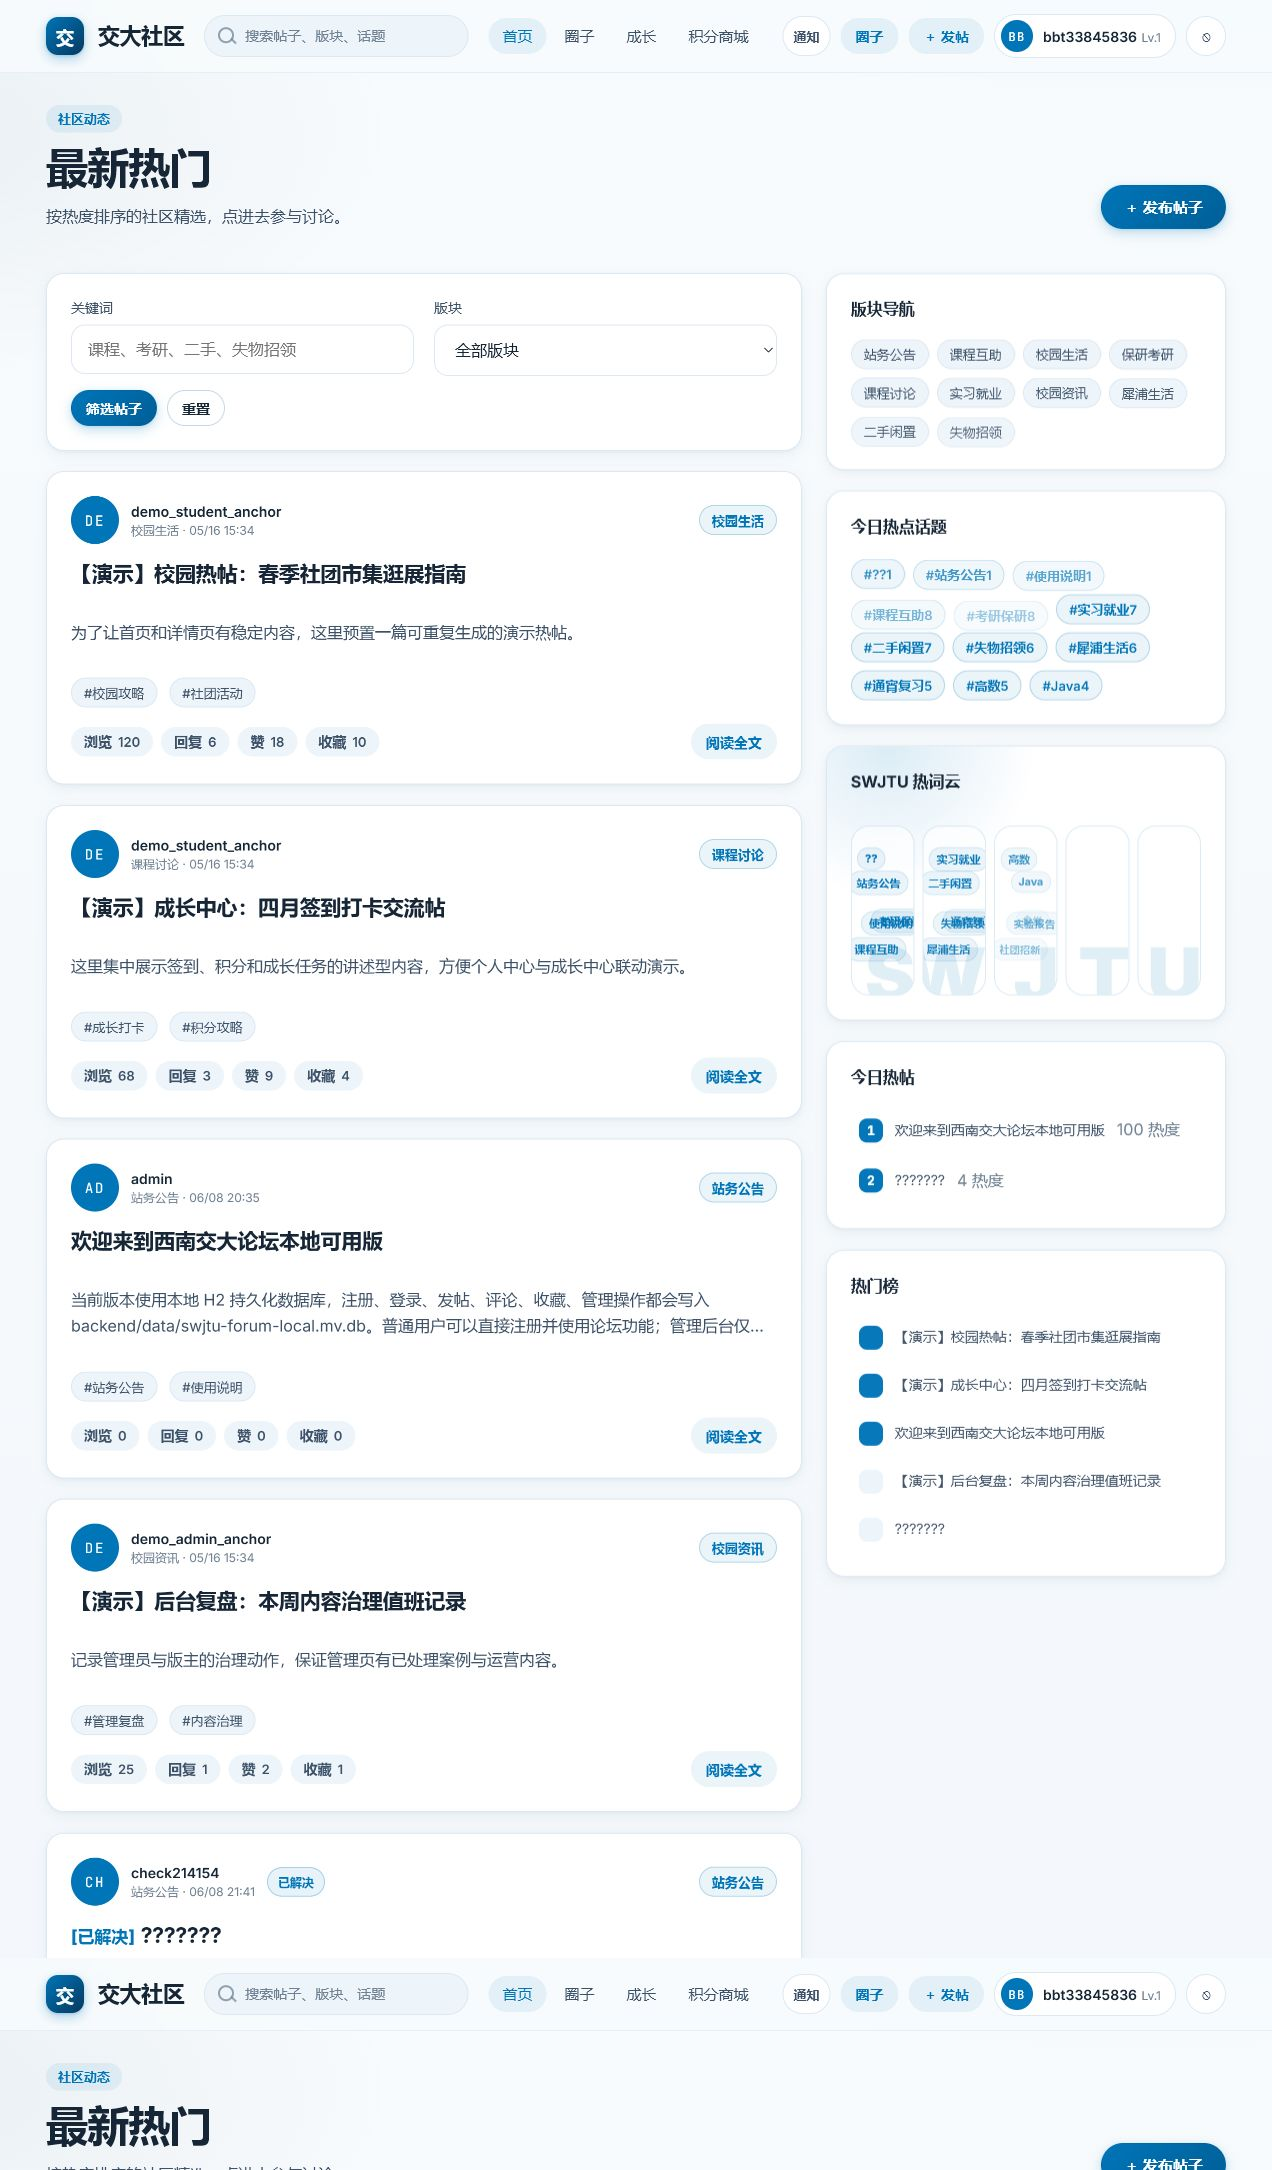
\includegraphics[width=0.82\textwidth,height=0.32\textheight,keepaspectratio]{figures/forum_test/05_home_post_list.png}
\caption{首页帖子列表与浏览入口}
\end{figure}

\subsection{发帖与评论流程}
执行步骤：使用已登录账号进入发布页面，填写标题、正文和版块，提交后进入帖子详情页，再继续检查评论输入框、点赞按钮和收藏按钮。断言点：详情页标题应与发布标题一致，评论区域可输入，互动按钮可见且不会遮挡正文。
\begin{figure}[H]
\centering
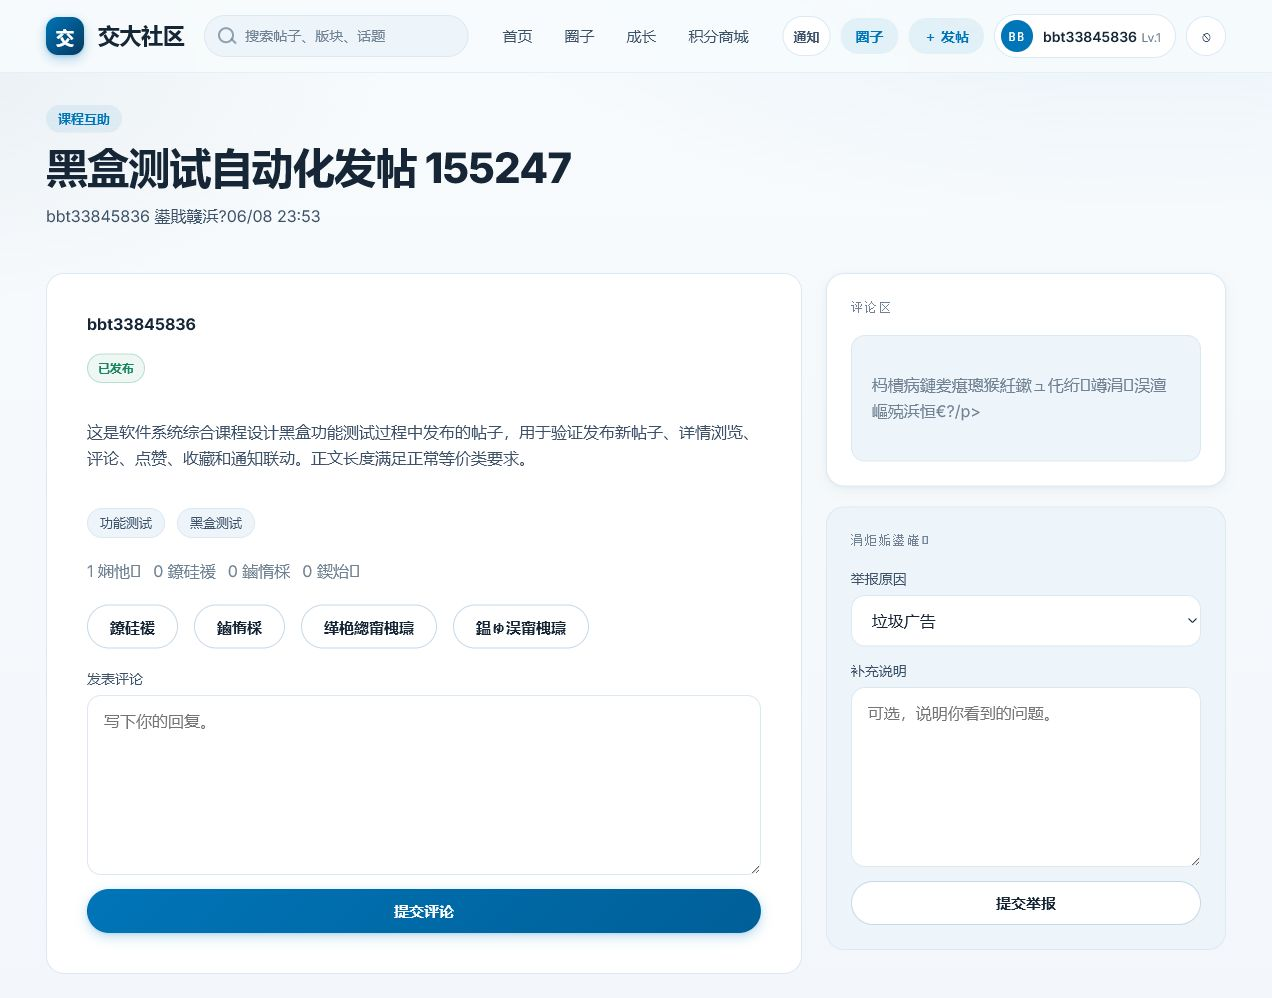
\includegraphics[width=0.82\textwidth,height=0.32\textheight,keepaspectratio]{figures/forum_test/09_create_post_success_detail.png}
\caption{发布帖子后进入详情页}
\end{figure}

\subsection{个人中心与身份信息流程}
执行步骤：进入个人中心后修改昵称、简介、学院和专业，保存后刷新页面，再进入校园身份认证区域检查身份信息。断言点：保存后的资料应继续显示，认证状态应与接口返回一致，长简介不应破坏页面布局。
\begin{figure}[H]
\centering
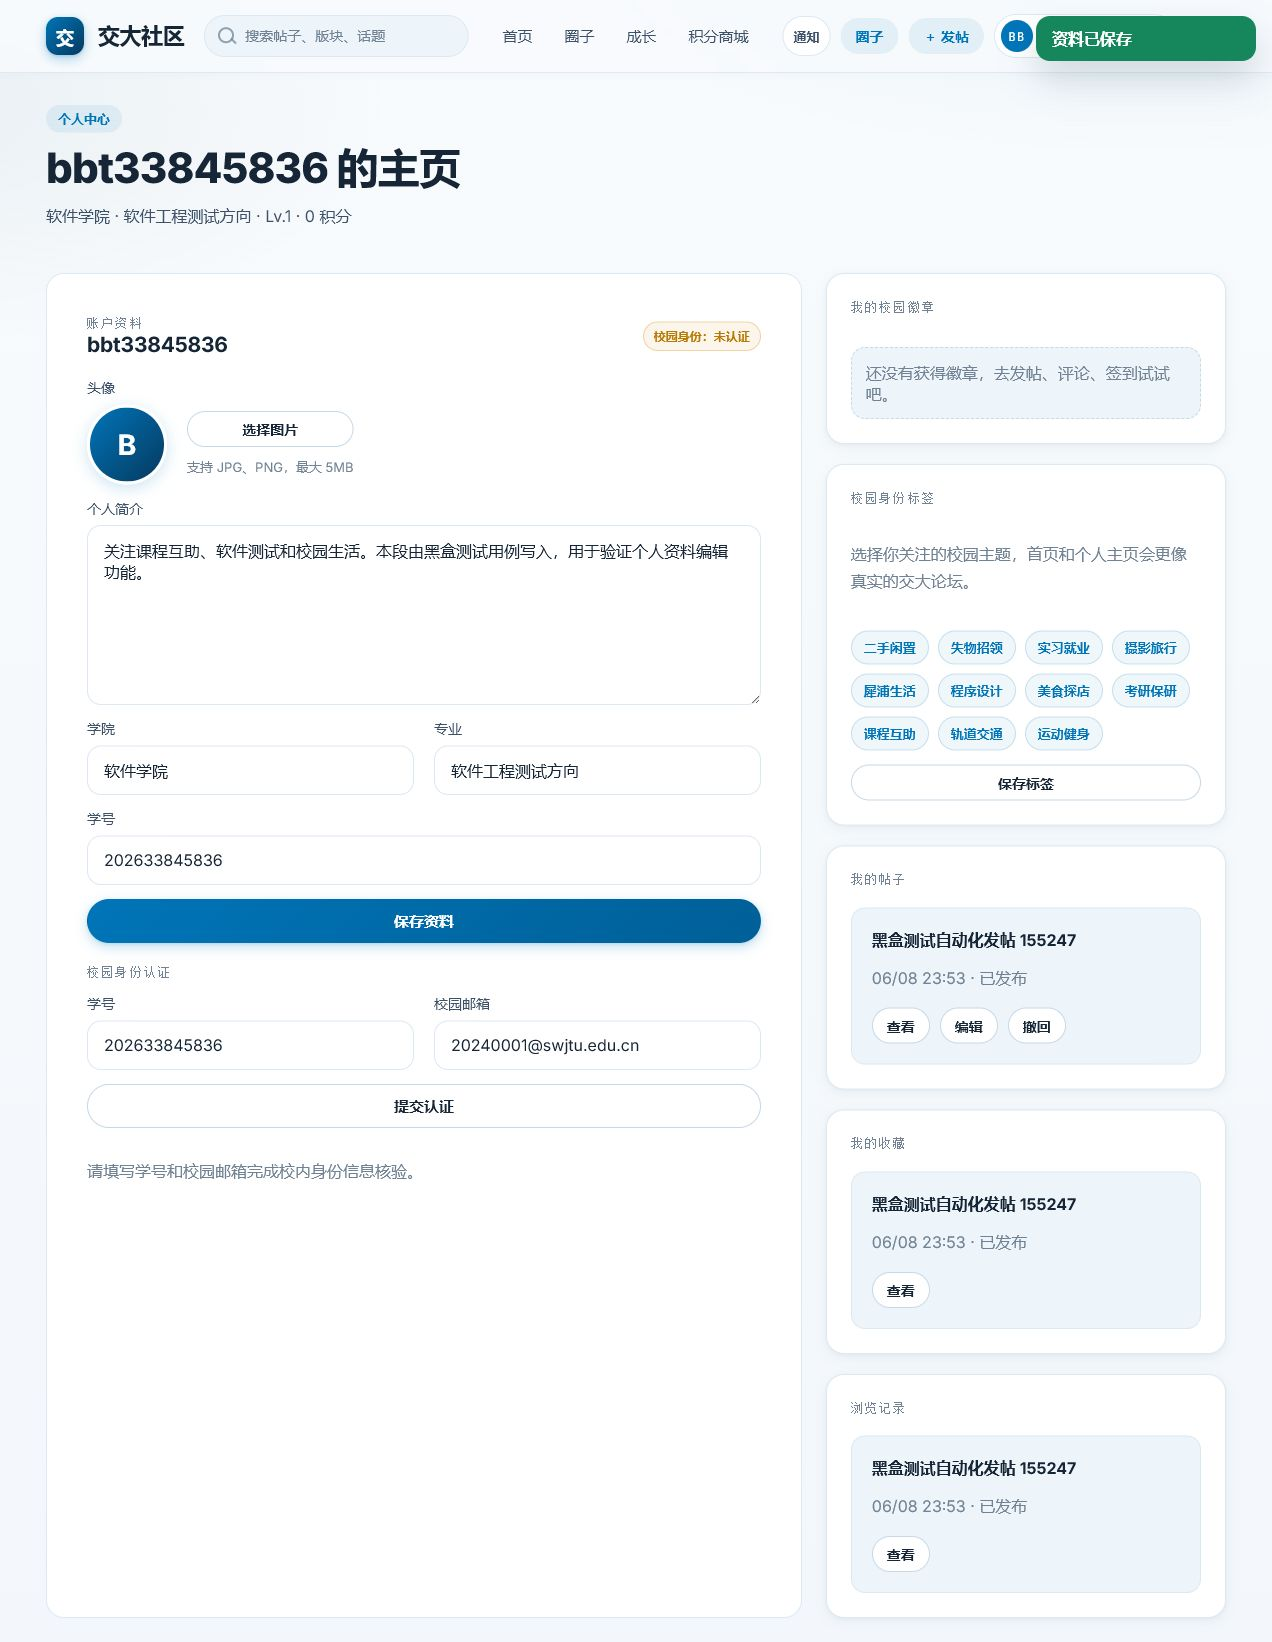
\includegraphics[width=0.82\textwidth,height=0.32\textheight,keepaspectratio]{figures/forum_test/14_profile_edit_success.png}
\caption{个人资料编辑后的页面状态}
\end{figure}

\subsection{积分商城与成长流程}
执行步骤：先查看当前积分和签到记录，再进入积分商城读取奖品卡片、所需积分和兑换按钮。断言点：奖品列表应正常渲染，积分不足时应给出业务提示，页面刷新后不应出现加载失败。
\begin{figure}[H]
\centering
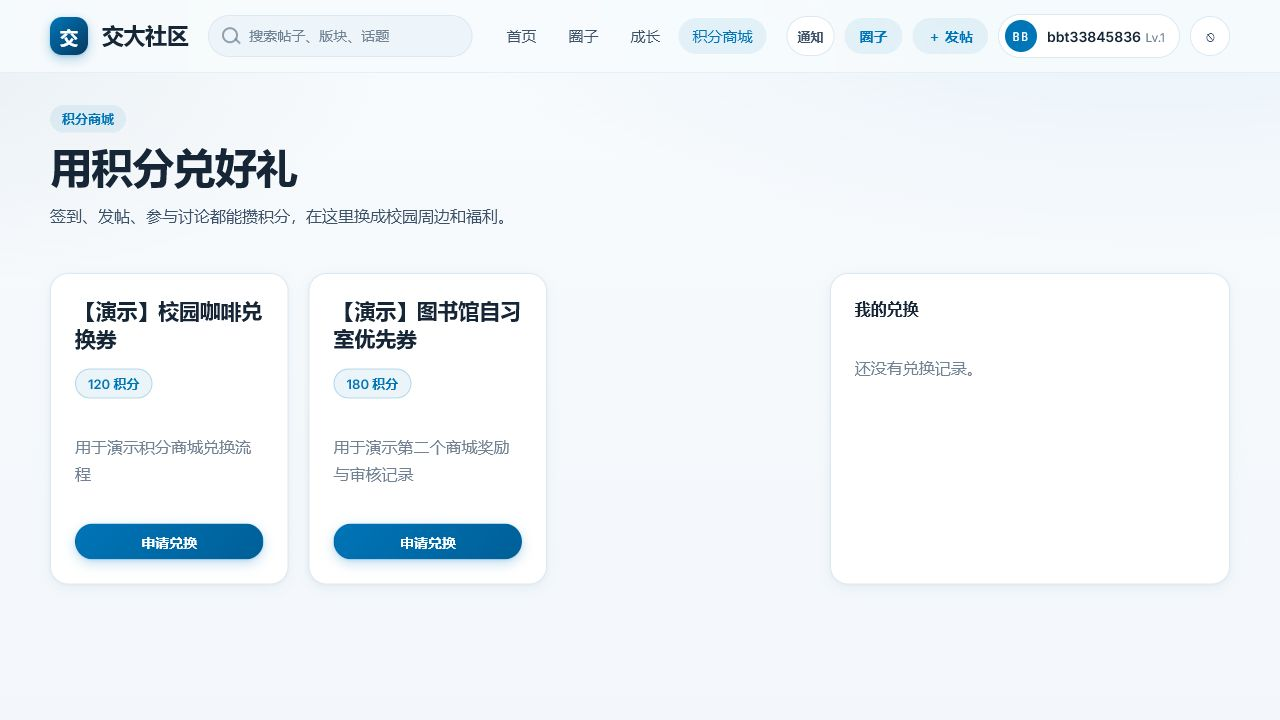
\includegraphics[width=0.82\textwidth,height=0.30\textheight,keepaspectratio]{figures/forum_test/20_rewards_mall_before_redeem.png}
\caption{积分商城奖品列表}
\end{figure}

\subsection{通知中心流程}
执行步骤：从页面右上角点击通知入口，等待通知面板出现，再读取通知标题、正文摘要和未读状态。断言点：面板应处于可见状态，通知内容能够被用户看到，未读数量或已读状态可以正常读取。
\begin{figure}[H]
\centering
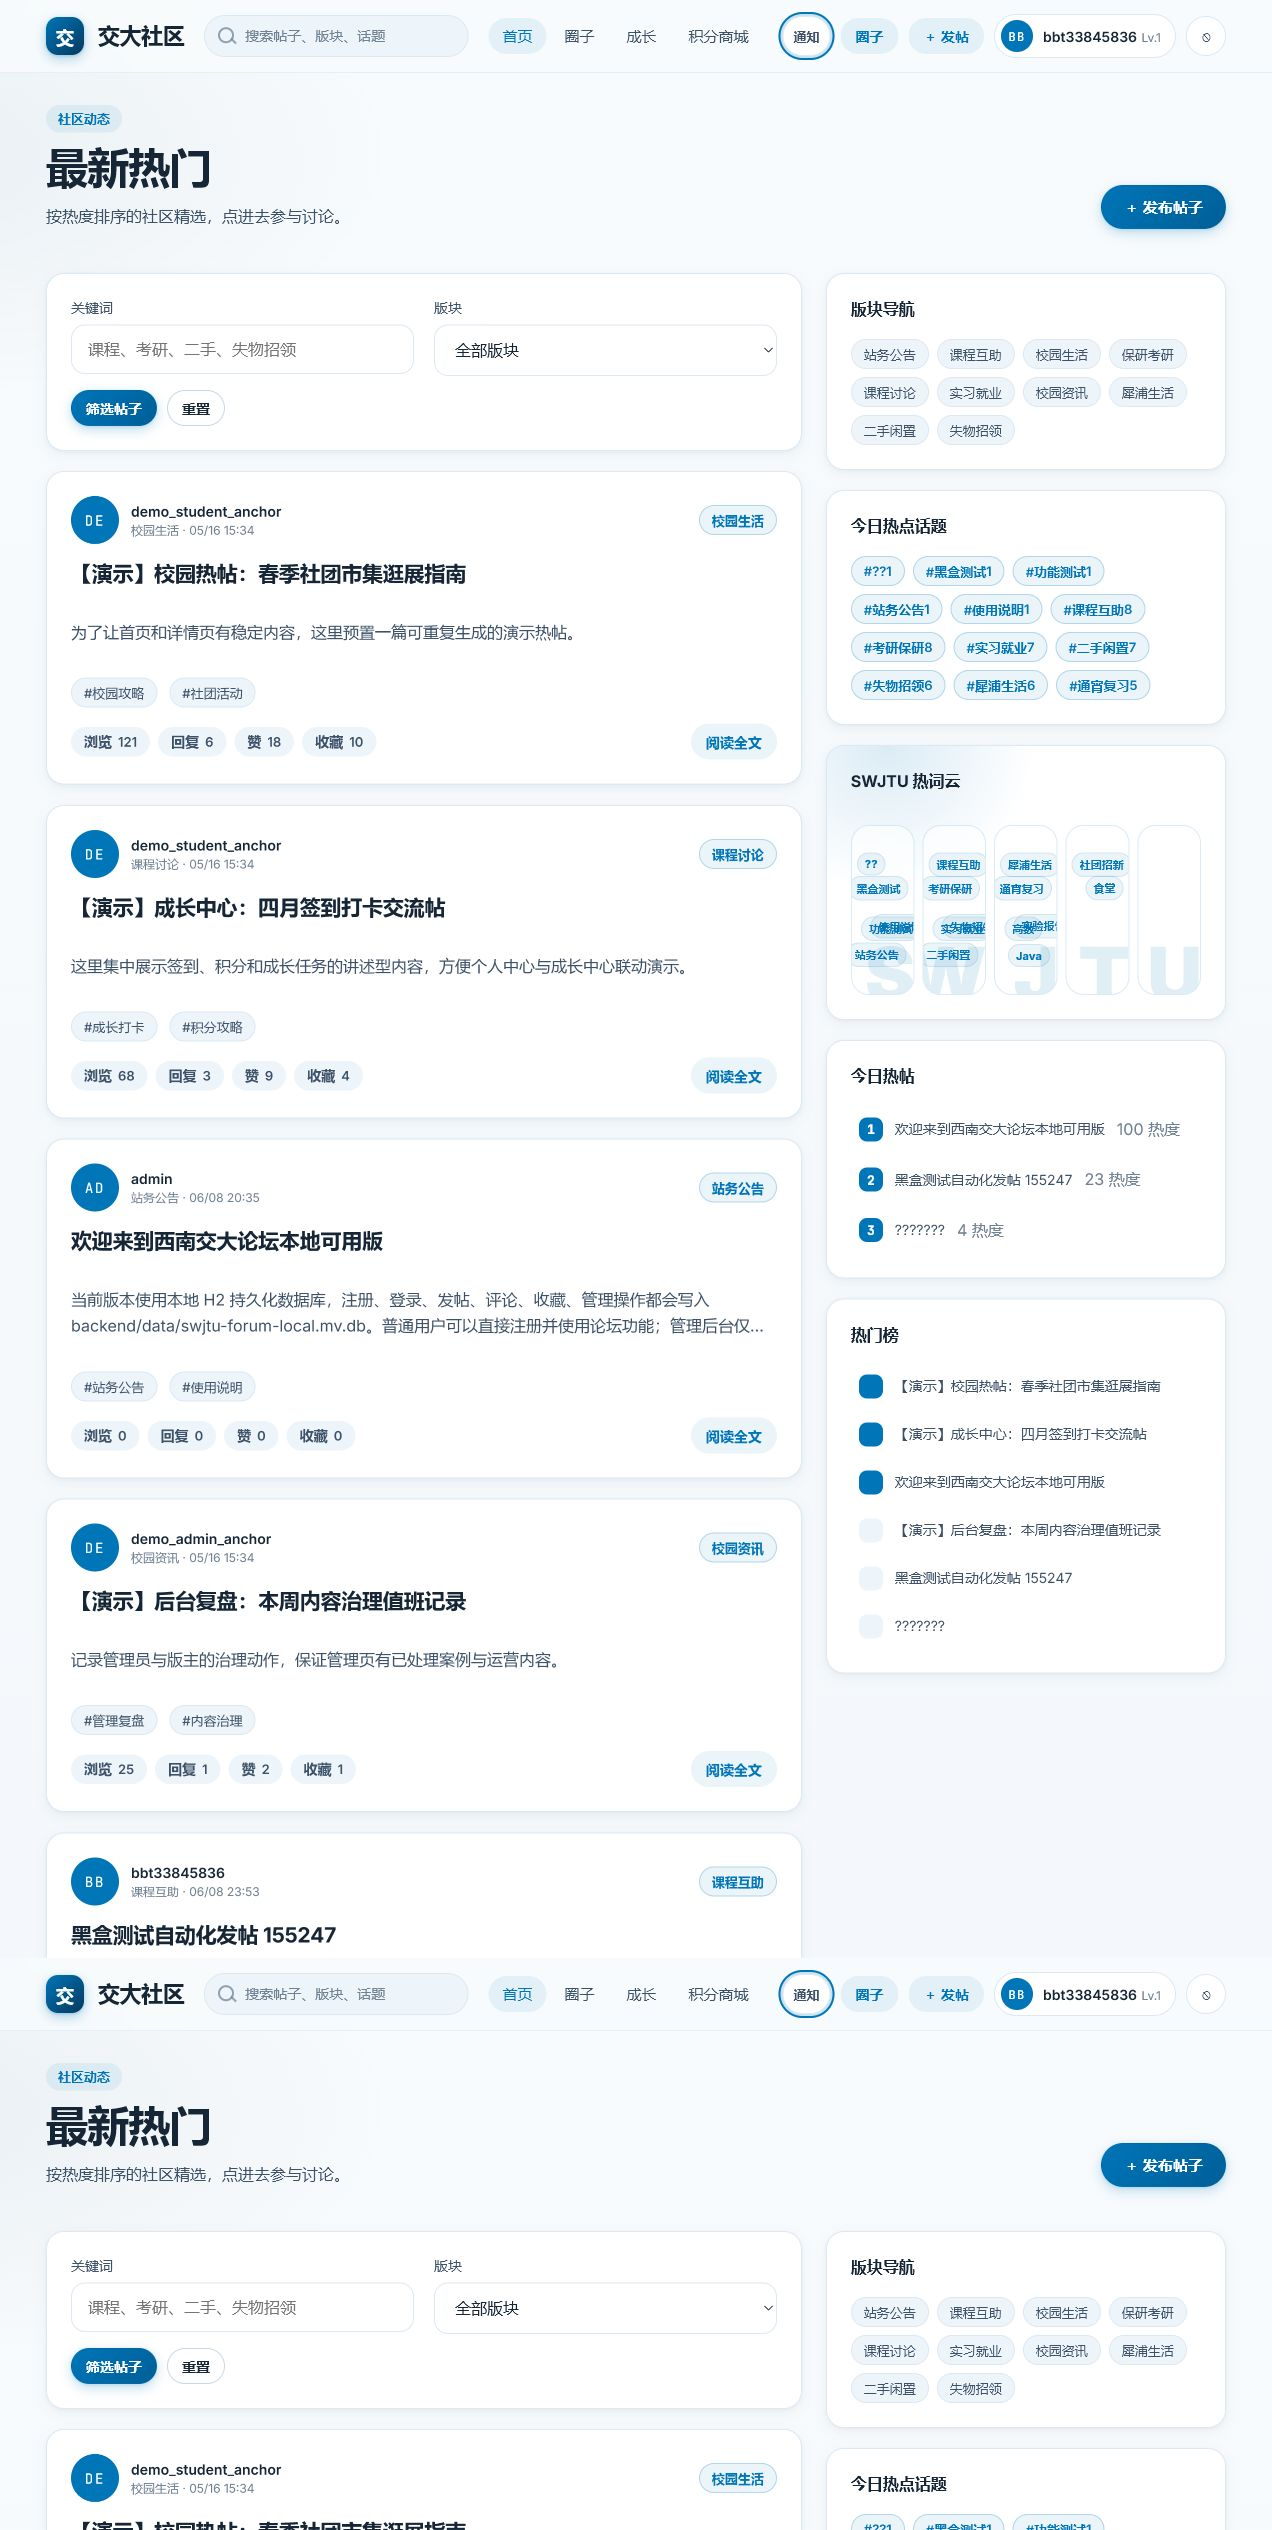
\includegraphics[width=0.82\textwidth,height=0.32\textheight,keepaspectratio]{figures/forum_test/22_notification_center_open.png}
\caption{通知中心展开后的页面状态}
\end{figure}

\subsection{关注关系流程}
执行步骤：进入帖子详情页，在作者信息区域点击关注按钮，记录按钮状态变化，再执行取消关注。断言点：关注后按钮状态应发生变化，取消后能回到初始状态，未登录用户不应直接建立关注关系。
\begin{figure}[H]
\centering
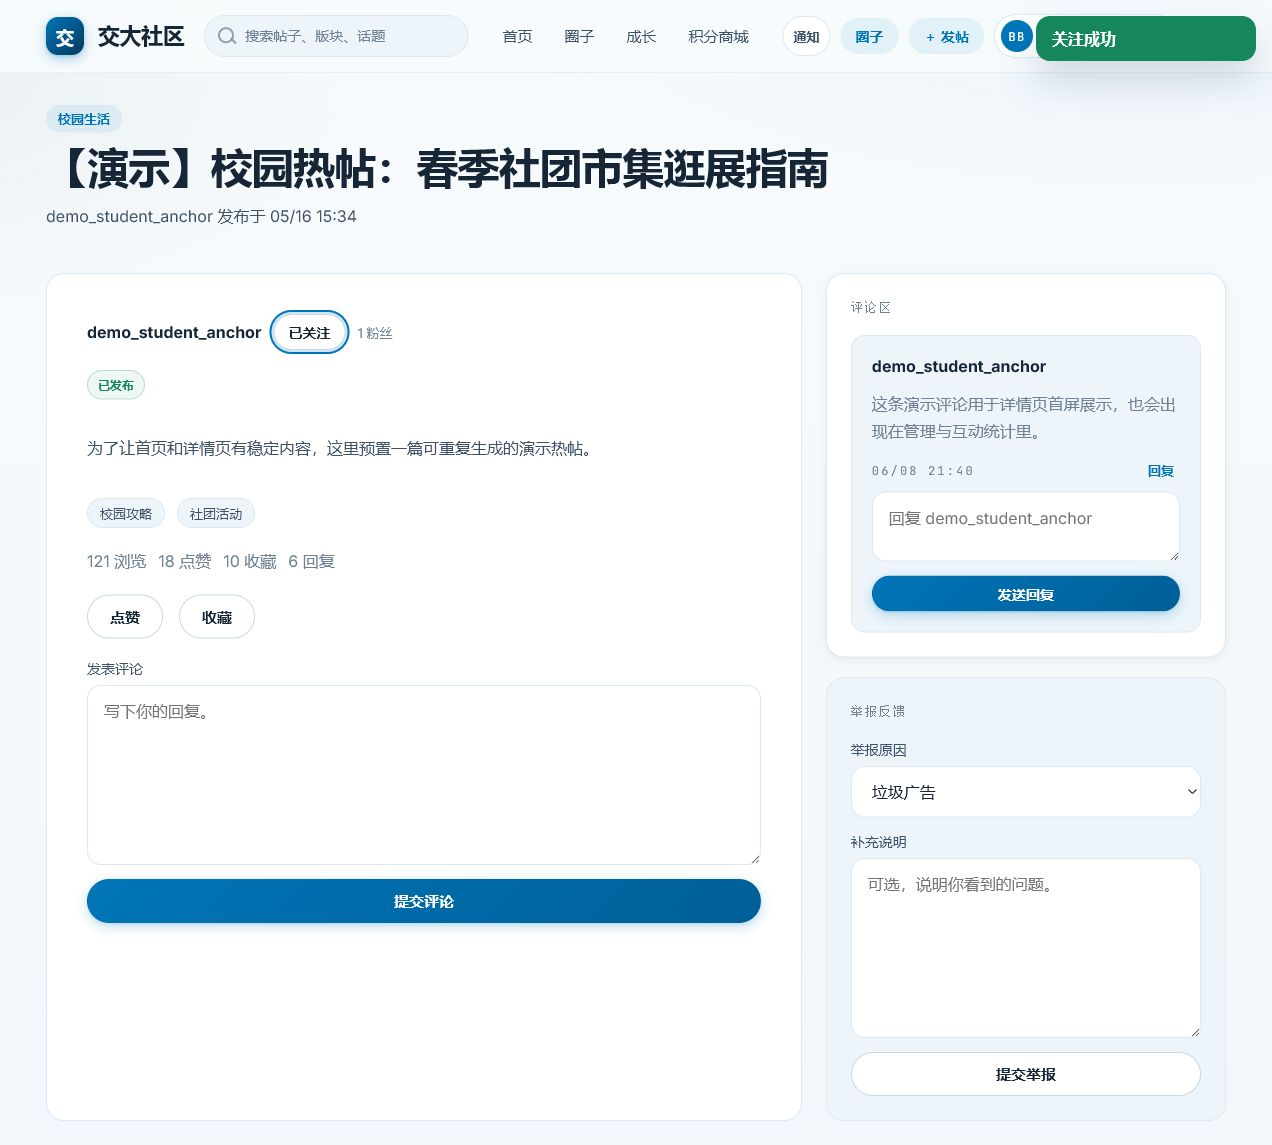
\includegraphics[width=0.82\textwidth,height=0.30\textheight,keepaspectratio]{figures/forum_test/24_follow_success.png}
\caption{关注用户后的页面状态}
\end{figure}

\section{测试结果分析与体会}
\subsection{通过用例分析}
本轮 75 条用例中通过 70 条，说明系统的核心业务闭环已经具备可用性。注册和登录链路能够完成新用户创建、管理员登录和登录态查询；首页列表、版块筛选和帖子搜索能够返回稳定结果；评论、点赞、收藏和关注能够在登录态下完成状态变化；个人资料、每日签到、积分商城列表、通知列表和未读数等接口也能在常规输入下返回合理数据。

\subsection{失败用例分析}
失败的 5 条用例不是平均分布在所有模块中，而是集中在三类问题上。第一类是主流程中断，例如发帖接口异常会直接阻止用户发布内容；第二类是业务规则不清，例如校园认证对不存在学号的处理不符合预期，覆盖资料前也缺少二次确认；第三类是展示一致性问题，例如详情页中文乱码和签到积分展示不一致。这样的分布说明基础浏览和互动链路较稳定，但涉及数据写入、身份资料覆盖和积分解释的路径仍需要继续处理。

\subsection{课程体会}
通过这次测试可以明显感受到，黑盒测试不是简单点击页面，而是从用户角度建立输入、状态和输出之间的映射。一个按钮能点击并不代表功能正确，一个接口返回成功也不代表业务完整。等价类帮助选择代表输入，边界值帮助发现长度和格式问题，判定表帮助覆盖多条件组合，自动化脚本则提高了回归效率和复核稳定性。


\appendix
\section{自动化测试脚本核心代码}
本附录列出浏览器自动化测试中的核心断言片段，主要用于说明等待、点击、可见性判断和页面内容检查的实现方式。脚本在 JUnit 5 中按用例顺序执行：启动浏览器后先完成管理员或测试用户登录，再进入对应页面；每次点击前使用显式等待定位元素，点击后重新读取 DOM 状态；断言失败时根据 JUnit 输出定位到具体测试方法，并结合页面截图或页面文本判断是脚本等待问题还是业务页面问题。

\begin{lstlisting}[language=Java,caption={通知中心可见性检查核心片段}]
@Test
@Order(2)
void notificationPanelMustBecomeVisible() {
    loginAsAdmin();
    driver.get(BASE_URL + HOME_PAGE);
    wait.until(ExpectedConditions.visibilityOfElementLocated(By.cssSelector("[data-notif-toggle]")));
    click(By.cssSelector("[data-notif-toggle]"));
    WebElement panel = wait.until(ExpectedConditions.presenceOfElementLocated(By.cssSelector("[data-notif-panel]")));
    Boolean hidden = (Boolean) ((JavascriptExecutor) driver)
        .executeScript("return arguments[0].hidden;", panel);
    String display = (String) ((JavascriptExecutor) driver)
        .executeScript("return getComputedStyle(arguments[0]).display;", panel);
    assertFalse(hidden, "notification panel should not be hidden after clicking bell");
    assertNotEquals("none", display, "notification panel display should not be none");
    assertEquals("true", driver.findElement(By.cssSelector("[data-notif-toggle]"))
        .getAttribute("aria-expanded"));
}
\end{lstlisting}

\begin{lstlisting}[language=Java,caption={积分商城页面刷新检查核心片段}]
@Test
@Order(3)
void rewardsAndRedemptionsMustLoadWithoutServerError() {
    loginAsAdmin();
    driver.get(BASE_URL + REWARDS_PAGE);
    wait.until(ExpectedConditions.not(
        ExpectedConditions.textToBePresentInElementLocated(By.cssSelector("body"), "页面加载失败")));
    assertFalse(driver.getPageSource().contains("Internal Server Error"));
    assertTrue(driver.getPageSource().contains("积分")
        || driver.findElements(By.cssSelector("[data-redeem]")).size() > 0);
}
\end{lstlisting}

\end{document}
